% Metódy inžinierskej práce

\documentclass[10pt,twoside,slovak,a4paper]{article}

\usepackage[slovak]{babel}
%\usepackage[T1]{fontenc}
\usepackage[IL2]{fontenc} % lepšia sadzba písmena Ľ než v T1
\usepackage[utf8]{inputenc}
\usepackage{graphicx}
\usepackage{url} % príkaz \url na formátovanie URL
\usepackage{hyperref} % odkazy v texte budú aktívne (pri niektorých triedach dokumentov spôsobuje posun textu)

\usepackage{cite}
%\usepackage{times}

\pagestyle{headings}

\title{Autopilot\thanks{Semestrálny projekt v predmete Metódy inžinierskej práce, ak. rok 2021/22, vedenie: Vladimír Mlynarovič}} % meno a priezvisko vyučujúceho na cvičeniach

\author{Samuel Švec\\[2pt]
	{\small Slovenská technická univerzita v Bratislave}\\
	{\small Fakulta informatiky a informačných technológií}\\
	{\small \texttt{xsvecs@stuba.sk}}
	}

\date{\small 6.11.2021} % upravte



\begin{document}

\maketitle

\begin{abstract}
Tento článok bude o tom ako funguje autopilot v lietadlách či v lodiach a taktiež pokrok v automobilovom priemysle. Rozoberie aj aktuálne chyby v softvéroch, ktoré môžu ovplyvniť spoľahlivosť a bezpečnosť autopilota a tým aj zastaviť používanie daného softvéru.
\end{abstract}

Kľúčové slová: autopilot, chyby, história

\section{Úvod}

Autopilot nie je v dnešnej dobe nový pojem. S autopilotom sa vieme stretnúť aj v našom bežnom živote, a to napríklad v leteckej či vodnej doprave. V oblasti automobilového priemyslu však nie je dostatočne autopilot využívaný. V súčasnej dobe niekoľko popredných firiem pracuje na vytvorení dokonalého automobilového autopilota, ako napríklad Tesla. Avšak, použitie autopilota prináša aj veľa hrozieb. 

Základný problém, ktorý bol naznačený v úvode, je podrobnejšie vysvetlený v časti~\ref{AFA}.
Ďalej je to rozvinuté v časti~\ref{chyby}.


\section{Autopilot v leteckej doprave} \label{AFA}

\subsection{História autopilota v letectve} 

Autopilot je technický systém, ktorý je počas prevádzky schopný zastúpiť človeka v riadení ovládaného objektu bez ďalšej ľudskej asistencie. Historicky prvý funkčný autopilot bol zostrojený v roku 1912 Lawrencom Sperrym, predstavený však bol verejnosti prvý raz až v roku 1914 a uvedený do prevádzky v lodnej doprave.\cite{AVA} Na obr.~\ref{f:obr2} môžeme vidieť vynálezcu Lawrenca Sperryho.

\begin{figure*}[tbh]
\centering
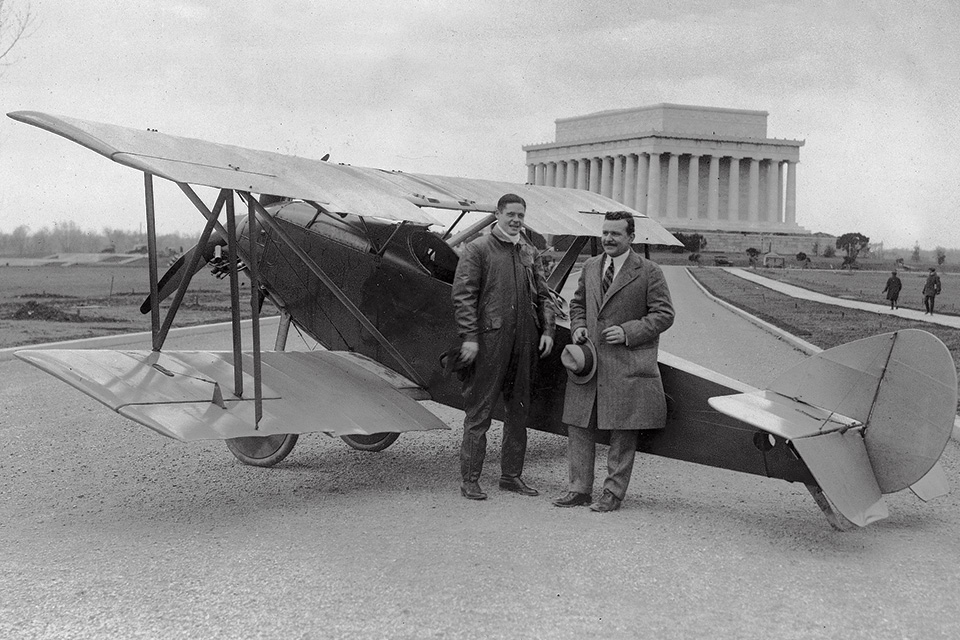
\includegraphics[scale=0.30]{obr2.jpg}
\caption{Lawrence Sperry (naľavo) - prvý funkčný autopilot}
\label{f:obr2}
\end{figure*}

\subsection{Autopilot v lietadlách} \label{AVL}
V letectve sa často stretávame s pomenovaním AFCS.\footnote{Automatic Flight Control Systems - automatické systémy riadenia letu}Tieto systémy sú univerzálne používané v komerčnom letectve. Rozsiahle uplatnenie nachádzajú aj vo vojenskom a všeobecnom letectve, ale koncepcia voľného letu, v rámci ktorej bude v budúcnosti prebiehať plne automatický let, je v podstate zameraná na zníženie preťaženia dýchacích ciest, čo je situácia, ktorá ovplyvňuje najmä komerčné letectvo. Hoci lietadlá všeobecného letectva wm musia tiež pracovať v prostredí voľného letu, väčšina týchto lietadiel má buď iba manuálne riadiace systémy, alebo je inštalácia AFCS len základná.\cite{AVA}

Hlavným účelom použitia AFCS je do určitej miery automatizovať lietanie lietadla, aby sa znížila pracovná záťaž pilotov (zvyčajne v určitej kritickej fáze letu), aby sa zachovala bezpečnosť letu. Čoraz častejšie sa AFCS používajú aj na zlepšenie základných letových vlastností lietadla (napr. na zabezpečenie dynamickej stability, aj keď bolo lietadlo navrhnuté ako staticky nestabilné), alebo na overenie základných výkonov lietadla v niektorých atmosférických podmienkach. Na dosiahnutie plne automatického letu bude potrebné, aby sa dosiahlo niekoľko dôležitých technologických a operačných systémových vývojov, ale vždy, keď sa to podarí, výsledný plne automatický systém bude fungovať prostredníctvom už vyvinutého AFCS.\cite{AFCS}

\begin{figure*}[tbh]
\centering
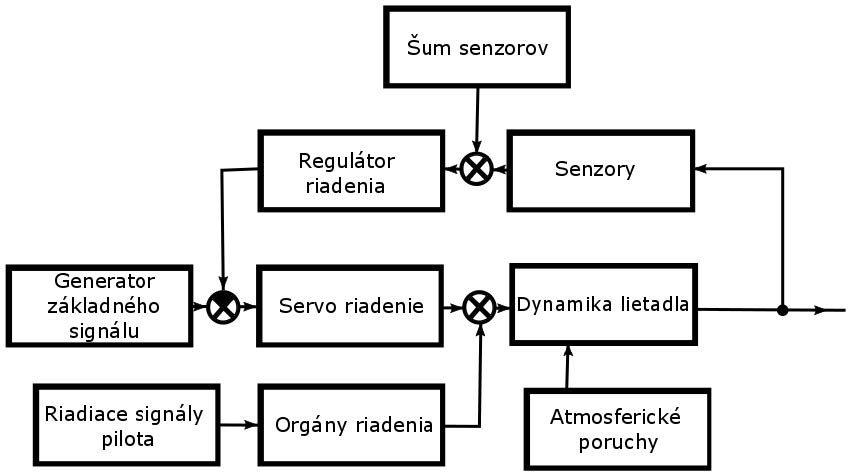
\includegraphics[scale=0.9]{obr1.jpg}
\caption{Funkčná schéma autopilota}
\label{f:obr1}
\end{figure*}

\section{Autopilot v automobiloch}

V následujúcej kapitole bude opísaný vývoj autonómnej jazdy v plne elektrických autách značky Tesla až po súčastnosť.

\subsection{Počiatky autopilota v automobiloch značky Tesla}

V roku 2014 bol predstavený prvý polo-autonómny autopilot. Bol to asistent parkovania, ktorý fungoval tak, že ovládal volať a jeho úlohou bolo vmanévrovať auto na parkovacie miesto, zatiaľ čo vodič mal na starosti ovládanie prídávať plyn a brzdiť automobil. 

Prvý autonómny autopilot predstavila automobilka Tesla v roku 2015. Autopilot vedel prebrať ovládanie vozidla. Autopilot sa staral o riadenie vozidla a taktiež oproti predchádzajúcej verzií autopilota aj o plynový a brzdový pedál. Avšak, vodič automobilu musel stále dávať pozor na premávku. Kvôli príliš vysokej dôvere autopilotu však dochádzalo k dopravným nehodám. Preto Tesla zakázala používanie tejto verzie autopilota.

Napriek tomu daná verzia autopilota bola schopná pomocou mobilnej aplikácie vyparkovať automobil z parkovacieho miesta a priviezť auto k vodičovi bez zásahu vodiča. Tento systém sa nazýva \emph{Summon}\footnote{ovládanie automobilu aplikáciou mimo vozidla}a dodnes je Teslou podporovaný.

V roku 2016 nastal veľký prelov v autopilote od automobilky Tesla. Predstavili autopilota, ktorý dokázal stále dávať pozor na premávku okolo automobilu, zvládol riadiť automobil v jednoduchých dopravných situáciach, akou je napríklad dopravná zápcha. \cite{TeslaAutopilot}

\subsection{Tesla Autopilot v dnešných dňoch}

V súčastnosti je automobil schopný prebrať riadenie na diaľnici alebo aj zaparkovať bez zásahu vodiča. Tento systém je nazvaný \emph{Parkseek mode}. Po vystúpení z auta nájsť voľné parkovacie miesto a zaparkovať. Následne ho pomocou mobilnej aplikácie jednoducho privolať k sebe. 

Ďalšou novinkou je aj takzvaný Supercharger. Je to špeciálna možnosť automatického nabíjania. Auto sa odstaví pri stojan, ktorý sám pripojí nabíjací kábel. Na stanici Supercharger trvá nabitie batérie automobilu ohruba okolo 30 minút. \cite{TeslaAutopilot}

\section{Adaptívne riadenie distribuovaných aplikácií autopilotu} \label{ARDAA}

Aj keď sa programovacie modely aj paralelné počítačové systémy naďalej rýchlo vyvíjajú, väčšina analýz výkonnosti zostáva založená na procese vyvinutom pred viac ako štyridsiatimi rokmi


\section{Chyby autopilota} \label{chyby}
\section{Zhrnutie}

\bibliography{literatura}
\bibliographystyle{plain} 
\end{document}